\DiaryEntry{Tilings}{2016-06-08}{Maths}

Consider a sequence \(l_n = 4n-3\). The first elements are
\(l_1=1, l_2=5, l_3=9, l_4=13,\ldots\). We are interested in the partial
sum

\[
S_N = \sum_{n=1}^N l_n
\]

An interpretation of the \(l_n\)s is shown in the Figure below: The
\(l_n\)s correspond to the number of squares in the same color: \(l_1\)
corresponds to the black square, \(l_2\) corresponds to the green
squares, \(l_3\) corresponds to the red squares, and \(l_4\) corresponds
to the blue squares.

\begin{figure}[H]
\centering
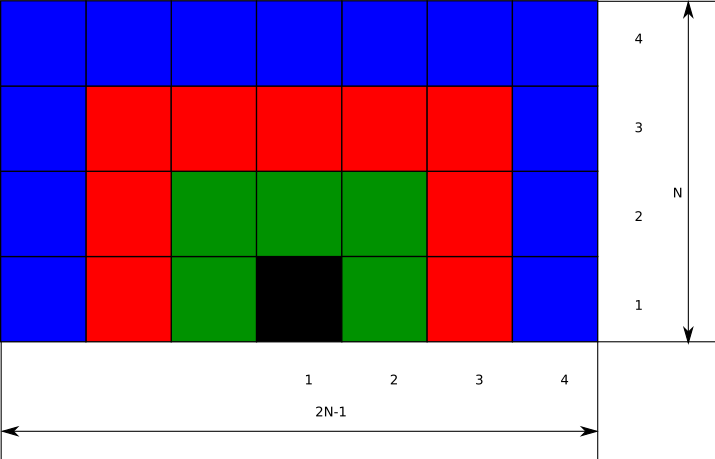
\includegraphics[scale=0.5]{images/tilings_01.png}
\end{figure}

The partial sum \(S_N\) is then the total number of squares contained in
a rectangle of width \(2N-1\) and height \(N\); therefore

\[
S_N = (2N-1)N
\]

and we deduce the following identity

\[
\sum_{n=1}^N 4n-3 = (2N-1)N
\]
